\section*{Introdution}

\begin{frame}
\frametitle{Qu'est-ce que GTD?}
\emph{Getting Things Done, the art of stress-free productivity}, David Allen\\
M\'ethode de gestion des priorit\'es quotidiennes.\\
Les taches \`a  r\'ealiser sont vues selon deux axes : par contexte ou par projet.\\
\begin{description}
\item[Contexte]environnement de travail (outils et lieu)
\item[Projet]objectif \`a atteindre (Passer un examen)
\end{description}
Mettre un diag ici.
\end{frame}

\begin{frame}
\frametitle{Le projet multi-module}
Fonctionnalit\'es :
\begin{itemize}
\item Collecter
\item Organiser
\item Agir
\item Revoir
\end{itemize}
\pause
Architecture globale de l'application : \\
\begin{center}
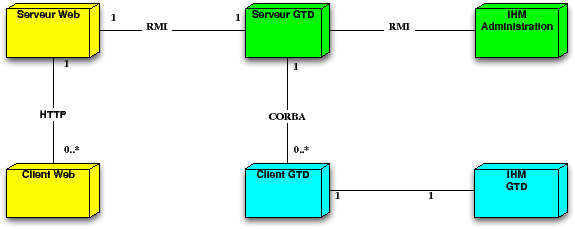
\includegraphics[width=8cm]{images/archi_gen}
\end{center}
\end{frame}